%Intro
With the increasing number of security and data breaches, individuals and organizations are far more concerned about their digital security and their data privacy. This is realized by the broadening discussion of data usage by companies and governments and their implications on privacy. Furthermore, this has reflected a growing demand for secure communication techniques in the various use cases of digital communication. Consequently, researchers and developers have been continuously seeking to improve the security features of algorithms and protocols and propose new ones rather than focusing solely on applications' features. Nevertheless, many deployed systems are built with alleged security guarantees, which are often violated. The reasons are the internal state compromises that occur through participants' exposures or the exploiting of newly discovered vulnerabilities in the presumed secure algorithms or protocols.
\par
A key compromise in message exchange algorithms that use the duplicate static keys for all messages allows an adversary to decrypt all messages. The long-term private key defines a party’s identity; thus, any compromise of the identity key can lead to an impersonation attack against its owner. A critical security feature of communication protocols is forward security which ensures the security of previous sessions if the current key is compromised. Nevertheless, the following question remains: Are there security guarantees for future sessions after a compromise? The security feature in question is referred to as backward secrecy, future secrecy, or post-compromise security. The ``future secrecy" term was composed by Marlinspike \cite{advanced_cryptographic_ratcheting_2013} in their discussion of an advanced ratcheting algorithm, while ``post-compromise security" was first coined by Cohn-Gordon et al. \cite{cohn2016post} in their definition and formal realization of the concept. In this thesis, we use the terms future secrecy and post-compromise security interchangeably since they are less confused with the forward secrecy property, from our point of view. According to \cite{cohn2016post}, post-compromise security is informally defined as ``A protocol between Alice and Bob provides Post-Compromise Security (PCS) if Alice has a security guarantee about communication with Bob, even if Bob’s secrets have already been compromised.". In the narrower context of long-term keys, it translates to that an algorithm is post-compromise secure if the compromise of a long-term key does not allow subsequent ciphered messages to be decrypted by passive attackers. Figure \ref{forward-future_secrecy} depicts the difference between forward secrecy and future secrecy.
\begin{figure}[htbp]
	\centering
	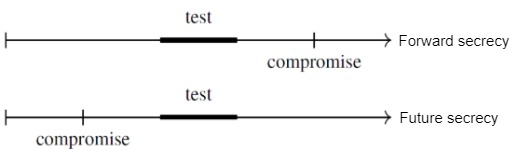
\includegraphics[scale=0.4]{Images/ffsecrecy.jpg}
	\caption[Forward and future secrecy]{Forward and future secrecy. Figure reproduced from \cite{cohn2016post}. The ``test" session indicates the session the adversary aims to attack. For either case, the aim of the security property is to guarantee security of the test session after compromise.}
	\label{forward-future_secrecy}
\end{figure}
Following the model of \cite{cohn2016post}, a client compromise can be broken down into weak compromise and total compromise. A weak compromise is when the client key is still private, however, the adversary has limited access to its usage. For example, an adversary can manipulate a compromised client to obtain a digital signature over data of his choice using the desired private key. On the other hand, a total compromise is more severe as the adversary learns the private key of the client and impersonate him without restrictions. Their work showed that future secrecy is achievable in both forms of compensation. Future secrecy in a weak compromise model is achievable if both parties can construct a secret in the ``test" session given that the adversary's access to the compromised key is revoked within that session. As for a total compromise model, future secrecy is achievable if both parties are capable of running a secure intermediate session where they construct a new intermediate secret before the ``test" session, where both secrets, the compromised and intermediate, are used in the ``test" session to derive a new secret. Likewise, the adversary's access to the compromised key is revoked in the intermediate and ``test" sessions.
\par
The Signal protocol is considerably one of the renowned instant messaging protocols with advanced security features \cite{unger2015sok}. It provides the critically desired forward and future secrecy, in addition to end-to-end encryption. Moreover, the protocol can be utilized in synchronous and asynchronous settings. Signal is composed of two main components: The \gls{x3dh} protocol \cite{x3dh} that is responsible for the initial \gls{ake}, and the double ratchet algorithm \cite{dblRtcht} that is responsible for generating secure message key in \gls{0rtt}. This chapter reflects on the details of the components of the signal protocol. We present a formal verification of \gls{x3dh} using OFMC. Neverthe less, we survey work done on formal verification of the Signal protocol and the post-quantum security of Signal.